\section{Actor-Critic with Experience Replay (ACER)}
\raggedbottom 

"Actor critic with experience replay" (ACER) introduced by \citet{ACER} was one of the first approaches to create a sample efficient, yet stable actor-critic method, that applies to both continuous and discrete action spaces.

ACER combines recent breakthroughs in the field of RL, by utilizing both the resource efficient parallel training of RL agents proposed by \citet{A3C} and the retrace algorithm \citep{Munos16}.

These approaches were combined with truncated importance sampling with bias correction and an efficient trust region policy optimization.
For continuous action spaces, stochastic dueling network architectures were used.

ACER can be viewed as an off-policy extension of A3C \citep{A3C}.
To understand the ACER-gradient, we start from the importance weighted policy gradient, which is given by:

\begin{align}
\hat{g}^{imp} = \left(\prod^k_{t=0}p_t\right) \sum^k_{t=0}\left(\sum^k_{i=0}\gamma^ir_{t+i}\right) \nabla_\theta \ log \ \pi (a_t \mid s_t)
\end{align}

A product of unbounded importance weights can cause high variance. \citet{Degris12} approached this problem by approximating the policy gradient as

\begin{align}
g^{marg} = E_{s_{t \textasciitilde{}} \beta, a_{t \textasciitilde{}} \mu} \left[p_t \nabla_\theta log \pi_\theta(a_t \mid s_t) Q^\pi (s_t,a_t) \left]
\label{gmarg}
\end{align}

where $\beta$ denotes the limiting distribution and $\mu$ the behaviour policy.

To compute this gradient, knowledge about $Q^\pi$ is necessary. We can use the retrace values (\ref{qretrace}) as a good estimation for $Q^\pi$.

To further reduce the variance, the importance weights are truncated.

By truncating the importance weights, bias is introduced.
Finding a good tradeoff between variance and bias is essential for the success of an RL-algorithm.
To counter this, ACER uses a bias correction term.

We will replace the importance weight $p_t$ in (\ref{gmarg}) with their truncated terms 

$\bar{p_t} = min \{ c,p_t \}$, where $c$ denotes the truncation value.

The introduced bias correction term is given as:

\begin{equation}
E_{x_t}\left[E_{a_{\textasciitilde{}\pi}} \left(\left[\frac{p_t(a) -c}{p_t(a)\right]}_+ \nabla_\theta log \pi_\theta(a \mid s_t) Q_\pi(s_t,a)\right)\right]
\end{equation}

To receive the ACER policy gradient we replace the $Q$ terms with our approximations. For the gradient term, the retrace values are used as an approximation, which further reduces variance in comparison to  using the estimated Q-function. $Q_\pi$ in the correction term is estimated by our critic.

Finally, we use the approximation of the value function, which is retrieved by taking the expectation of $Q_{\theta_v}$ under $\pi_\theta$ as a baseline by subtracting them from the Q terms.

This leaves us with the ACER policy gradient:

\begin{equation}
\begin{split}
g^{ACER}_t = \tilde{p}_t \nabla_\theta log \pi_\theta(a_t \mid s_t) \left[Q^{ret}(s_t,a_t) - V_\theta_v(s_t)\right] \\
+ E_{a_{\textasciitilde{}\pi}} \left(\left[\frac{p_t(a) -c}{p_t(a)\right]}_+ \nabla_\theta log \pi_\theta(a \mid s_t) \left[Q_\theta_v(s_t,a) - V_\theta_v(s_t)\right]\right)
\end{split}
\end{equation}

Note that the expectation over states is no longer necessary because it is approximated by sampling trajectories generated by $\mu$

The critic $Q_\theta_v$ is trained by minimizing the mean squared error with the retrace values as the target.

The critic loss function is given as: 

\begin{equation}
(Q^{ret} (s_t,a_t) - Q_{\theta_v} (s_t,a_t))^2 
\end{equation}

and has the standard gradient:

\begin{equation}
(Q^{ret}(s_t,a_t) -Q_{\theta_v}))\nabla_{\theta_v}Q_{\theta_v}(s_t,a_t))
\end{equation}

An entropy term of the policy $\pi$ is added to the optimization function to encourage exploration. 
Adding the entropy to our objective empirically performs better and can prevent early convergence to suboptimal policies.

The entropy for a policy $\pi$ is given by:

\begin{equation}
H(\pi) = -\sum^A_{i=1} \pi(a_i)\log_b \pi(a_i)
\end{equation}

where b denotes the basis for the logarithm. A common choice for the base is 2, 10 or e. \citep{entropy}

\citet{ACER} proposed an efficient trust region policy optimization (TRPO), which limits the update step in a way, that the new policy doesn't deviate too much from an average policy. 

Even though the TRPO method significantly improves the performance for continuous action space environments, the results presented in the paper only showed a marginal improvement for discrete action space environments.
TRPO comes with a relatively high computational cost in comparison to its benefits on the discrete action space.
Since only discrete action spaces were considered within this work, in order to conduct more experiments within the limitations of time and computational resources, the trust region optimization was not used.

Pseudocode for the algorithm used can be found at the end of the thesis (Algorithm \ref{ACERALGO}).

\subsection{Experimental Setup}

\subsubsection{Environment}
All experiments were made using multiple selected games from the Atari 2600 console game environments provided by \citet{openaigym}.

In our experiments the following OpenAI-Gym environments were used:

\textbf{Breakout} is a game that rapidly speeds up, making it easy for machines to show "superhuman" performance.

\textbf{Seaquest} poses a serious problem for learning agents, as they tend to get stuck on local maxima. It is especially interesting, as it provides multiple possibilities to achieve rewards.
The loss of the game if the player runs out of oxygen is a game mechanic a human can grasp in an instant, but it is notoriously hard for reinforcement learning agents to 'understand'.


\textbf{Space Invaders} is a fast-paced game. Human and reinforcement learning approaches for DQN achieved similar scores. \citep{mnih2015atari}

\textbf{Riverraid} is another game where humans manage to heavily outperform approaches like DQN.

The hyperparameters were adjusted to ensure a good performance for the Breakout environment. Tests on other environments were all performed with the same set of hyperparameters.


OpenAI gym environments provide the agent with a 210x160 pixel colored image. \linebreak
OpenAI uses a variation of the frame skipping method proposed by \citet{nature}.
Whenever the agent takes an action within the environment, instead of using it once and observing every state, the action is repeated over $k \in \{2,3,4\}$ game steps, and only every k'th observation is returned to the agent. Frame skipping reduces the workload of the agent and the length of the episodes, enabling a faster learning process.


\subsubsection{Preprocessing}
Using full scale colored images would come with a huge computational cost, resulting in a very slow learning process.
To make efficient use of the data, each frame is preprocessed.
First, the scoreboard area on top of the frame is chopped off, leaving roughly the playing area behind.

The playing area is then grayscaled and downscaled. With this method a 84x84 grayscaled pixel image is obtained.

Different grayscaling methods exist (Intensity, Luma, Lightness,...). Within this thesis, we worked with the luminance. It is given as

\begin{equation}
G_{Luminance} \gets 0.3 R + 0.59 G + 0.11 B,
\end{equation}

with R, G and B denoting the red, green and blue values.

\citet{nature} proposed to stack multiple frames. More specifically the state contains the last 4 frames received and therefore has a shape of 84x84x4.

To receive the initial state, we stack the first frame 4 times.
This can convey a feeling of movement to the agent.

\begin{figure}
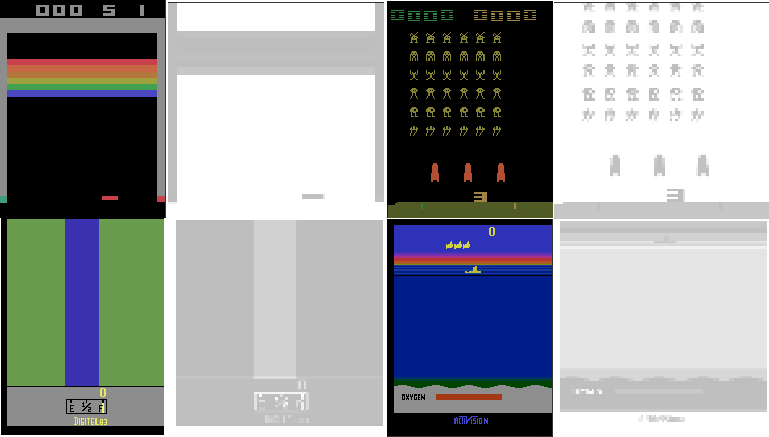
\includegraphics[scale=0.5]{bilder/atarienv.png}
\caption{The Atari 2600 console games Breakout, SpaceInvaders, Riverraid and Seaquest before and after being processed.}
\end{figure}

A high variance within the reward signal seems to negatively impact the learning of an agent.
A very common method to achieve good convergence is to limit the reward. 
It was found to be a good method to simply keep the sign of the reward, and ignore the magnitude, so rewards are either -1, 0 or 1. This method was adopted in this paper.


\subsubsection{Network Architecture}

Two architectures were tested. \citep{mnih2015atari} \citep{nature}.
Both provided good results. Since the paper uses the architecture proposed in the nature paper \citep{nature}, all further experiments were done using this architecture.

Similar to the A3C \citep{A3C} network, most of the parameters are shared and used for both estimating $Q^\pi$ and calculating the policy $\pi$.

The shared net consists of 3 convolutional layers.
First 32 8x8 filters are applied with a stride of 4.
The 2nd layer consists of 64 4x4 filters using a stride of 2.
The last convolutional layer uses 64 3x3 filters with stride 1.
Finally, a fully connected layer of size 512 is applied.

Each of the mentioned layers is followed by a rectifier nonlinearity (ReLU) function.
ReLU is used to set all negative outputs to 0, ensuring only positive values are passed to the next layer.

A test run using tanh instead of ReLU as activation function caused a significant loss of performance.

We map the final shared layer to the action space twice to obtain the action scores, and the Q-values. A softmax policy is used to receive the distribution over actions.
The action is then randomly sampled from the softmax probabilities.

\begin{equation}
P(A = a' | s ) = \frac{e^{z_\theta(a')}}{\sum^N_{i=0}e^{z_\theta(a_i)}} 
\end{equation}

where $z_\theta(a_i)$ denotes the score assigned to the i'th action through the last network layer.

\begin{figure}
\begin{center}

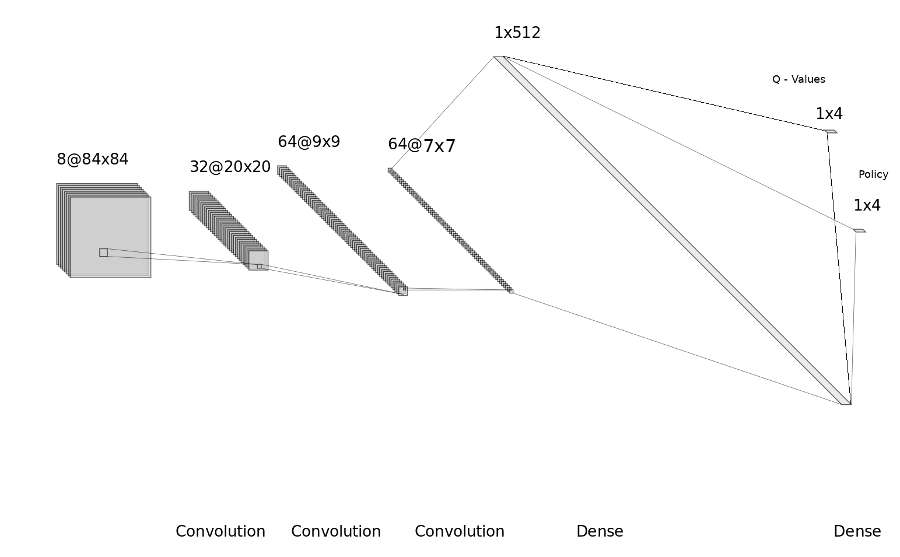
\includegraphics[scale=0.5]{bilder/nn2.png}
\caption{Shared network for policy and Q-Value approximization for an environment with 4 possible actions}
\end{center}

\end{figure}

The agent is trained by using 16 learner threads running on the CPU. Each thread has it's own replay buffer, which ensures a more balanced replay and reduces the risk of a single trajectory being used unreasonably often compared to a single shared replay buffer.

Updates to the network were performed every 20 steps or if the environment reached a terminal state. 

Replay buffers were designed to hold up to 2500 trajectories, therefore ~50.000 frames were saved for each thread and $_\tilde{}$ 800.000 frames were stored in total, which is the same size used by DQN \citep{nature}}

If no replay is used, ACER essentially becomes a version of A3C which uses retrace and Q-values, rather than learning the value function. \citep{A3C}

For the offline setting, replay ratios of 1, 2 and 4 were considered, where a ratio of 4 would mean, that the net is trained on trajectories sampled from the replay buffer 4 times for every online update.

The update was performed using an RMSProp Optimizer.
The RMSProp update is given by:
\begin{align}
g = \alpha g + (1- \alpha) \delta \theta^2 \\ \theta \gets \theta - \eta \frac{\delta \theta}{ \sqrt{g+\epsilon}}
\end{align}

where $\eta$ denotes the learning rate and $\alpha$ is the momentum. $\epsilon$ is a small value to prevent dividing by 0.

RMSProp has shown to be very robust for A3C. \citep{A3C}

A single optimizer is used for all threads, which gives a smoother momentum and shows better results compared to using a seperate optimizer for each thread.

Since RMSPropOptimizer in tensorflow, which was used for the implementation, can only use gradient decent, the following loss-function was minimized. Instead of having seperate updates for policy, value function and entropy, a single loss is formed and optimized.

\begin{equation}
L_{ACER} = - L_{Policy} + w_q L_{Q} - \beta Entropy
\end{equation}

with L denoting the loss. $w_q$ and $\beta$ are hyperparameters used to decide how much influence the value loss and the entropy should have on the parameters compared to the policy loss. Common values for $w_q$ are 0.5 or 0.25, whereas the entropy is usually weighted with 0.01 or 0.001.

\begin{figure}
\begin{center}

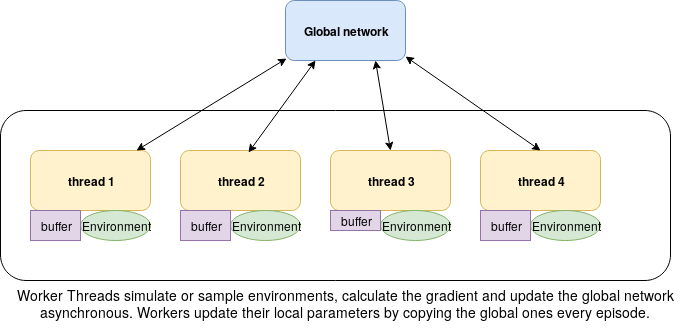
\includegraphics[scale=0.5]{bilder/ACERarchitecture.png}
\end{center}

\end{figure}
\pagebreak
\subsection{Hyperparameter settings}

Unless stated differently, the following hyperparameters were used.

\begin{tabular}{ |l|l|l| }
\hline
\multicolumn{3}{ |c| }{Hyperparameters} \\
\hline
Parameter & Value & Explanation  \\
\hline
LR & 8e-5 & learning rate \\
Discount & 0.99 & \\
return steps & 20 & \\
c & 10 & truncation value \\
$\beta$ & 0.01 & weight of entropy in the loss function \\
$w_q$ & 0.25 & weight of value loss. \\
RMSProp decay & 0.99 & \\
global norm & 10 & gradient clipping \\
$\epsilon$  & 1e-6 & clipping value denoting the distance to 0 and 1 \\ 
& & a probability is allowed to reach \\
\hline
\end{tabular}

\pagebreak
\section{Results}

The reward given in the graphics for the y-axis is the capped reward used to train the agent.
The actual reward achieved within the games will be discussed afterwards.
The decision to use the capped rewards was made due to their lower variance, and because these rewards were used when training the agent. 
The x-axis denotes the on-policy steps for the results on sample efficiency, and the computation time in terms of on-policy steps. In our experiments 100.000 on-policy updates on a CPU using 16 threads took about an hour.

\begin{figure}[h]
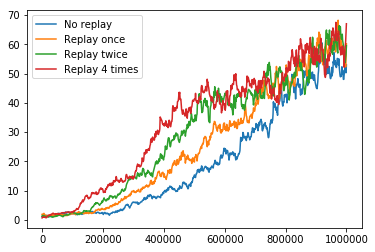
\includegraphics[scale=0.55]{bilder/breakoutbyonline.png}
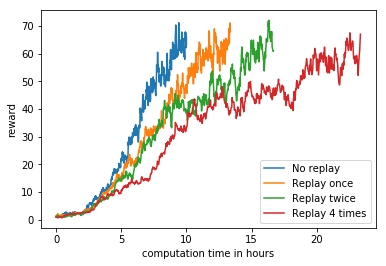
\includegraphics[scale=0.55]{bilder/breakoutbytime.png}
\caption{ACER results on the Breakout environment in regards to sample efficiency (left) and computation time (right).}
\end{figure}
\textbf{Breakout}

We can see that ACER is clearly more sample efficient with a higher replay ratio and quickly reaches better rewards. 
The right side shows the performance in regards to the computation time. Instead of looking at the actual time, we will instead consider the relation towards the online steps, since this does not depend on the hardware. During our experiments,  we found an online step to take about 3 times longer than an offline update.
In regards to the Breakout environment, we can conclude, that using a higher replay ratio (within the tested ratios) offers better performance in terms of sample efficiency, but can not match the learning speed of the online agent.


\begin{figure}[h]
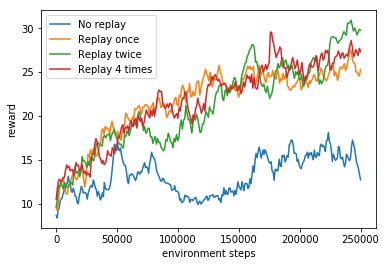
\includegraphics[scale=0.55]{bilder/spaceinvbyonline.png}
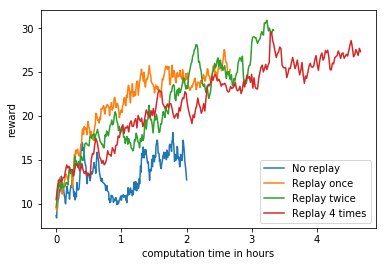
\includegraphics[scale=0.55]{bilder/spaceinvbytime.png}
\caption{ Results on Space Invaders in terms of sample effciency (left) and comutation time (right).}
\end{figure}

\pagebreak
\textbf{Space Invaders}

The poor performance of the online variant on Space Invaders came unexpected. Assuming this performance was caused by an unlucky initialization, the same test was performed again, but very simlar results were observed. In comparison, the agents using replay had a much smoother performance curve.
Unlike with the Breakout environment, a higher replay ratio did not result in a faster learning process.
\begin{figure}[h]
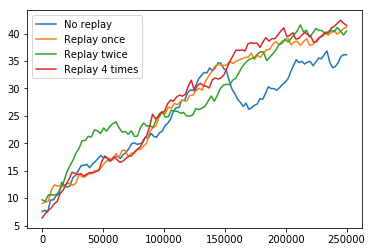
\includegraphics[scale=0.55]{bilder/seaquestbyonline.png}
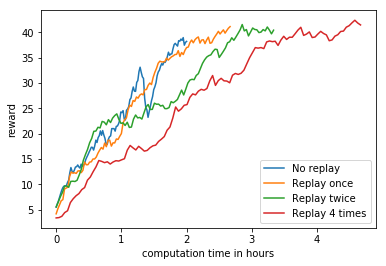
\includegraphics[scale=0.55]{bilder/seaquestbytime.png}
\caption{ACER results on the Seaquest environment in regards to sample efficiency (left) and computation time (right).}
\label{seafig}
\end{figure}

\textbf{Seaquest}

No significant performance increase in terms of sample efficiency could be observed. Independent of the replay ratio, all agents learned relatively even in terms of sample efficiency.
Using a replay ratio of 1 provided a smooth and efficient learning process in terms of both processing time and sample efficiency. \linebreak A significant drop in performance was observed for the online agent. In comparison all the replay agents providing a more smooth and stable learning process.
 

Even though the main purpose of ACER is to provide a sample efficient algorithm, it additionally seems to smoothen the learning process.
\begin{figure}[h]
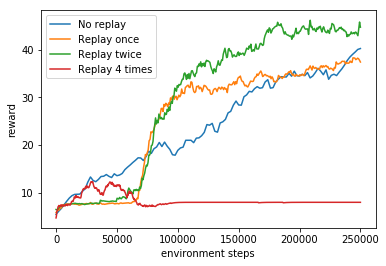
\includegraphics[scale=0.55]{bilder/riverraidbyonline.png}
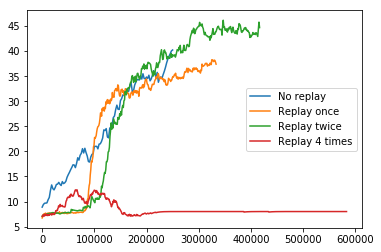
\includegraphics[scale=0.55]{bilder/riverraidbytime.png}
\caption{ACER results on the Riverraid environment in regards to sample efficiency (left) and computation time (right).}

\end{figure}

\textbf{Riverraid}

The experiments conducted on the Riverraid environment showed a rather slow learning in the beginning for the replay agents, with the replay ratio of 4 getting stuck on a low reward. A possible explanation could be, that the agent uses the trajectories sampled at the beginning of the learning process too often.

An attempt to fix this problem is to fill up a certain amount of the replay buffer first, and start the experience replay afterwards, to not reuse the same trajectory too often in the learning process. Sadly the Riverraid environment was the last environment to do experiments on, leaving us with little time to compare results with and without first filling up the replay buffer for different replay ratios and environments.

Even though the observed results showed better overall performance, the slow learning in the early phase remained

\begin{figure}[h]
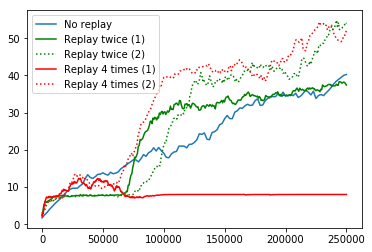
\includegraphics[scale=0.55]{bilder/riverraidreplayonline.png}
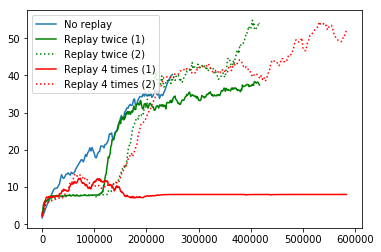
\includegraphics[scale=0.55]{bilder/riverraidreplaytime.png}
\caption{ACER results on the Riverraid environment in regards to sample efficiency (left) and computation time(right). (1) Uses replay throughout the full learning process. (2) Started replay after 1000 trajectories were saved to the buffer.}
\end{figure}

\pagebreak

\section{Preprocessing Atari Environments}

Atari environments were specifically designed for humans. Important information might be conveyed through text messages or symbols to a human, but might be heavily underrepresented within the pixel data.

A good examples for this problem is the Sequest environment. 

Seaquest often gets learning agents stuck on a local maximum because unlike a human they do not refill the oxygen.
A human player managed to outperform DQN \citep{nature} gaining four times the reward on average for Seaquest.
This is in line with the observations within this thesis. Figure \ref{seafig} shows the agents approaching a cap around 40 reward.

Even though future methods might overcome these problems, we can assume, that a well preprocessed environment will always outperform if compared with a poorly or non preprocessed environment.
Through smart preprocessing even very basic policy gradient methods can solve environments like Pong.  \citep{karpathy}

The core problem Seaquest has, is that the agent often cannot link the oxygen bar depleting to the end of the game. 
An attempt to increase the influence of the oxygen bar on the actions, could be to use space not relevant to the game to increase the size of the bar, therefore increasing its influence on the policy.
In addition, the hyperparameters for the return step: $k=50$ and $\gamma =0.995$ were adjusted to make future rewards more attractive to the learning agent.

\begin{figure}[h]

\includegraphics[scale=1]{bilder/seaquestgamenopre.png}

\includegraphics[scale=1]{bilder/seaquestgameprepro.png}
\caption{Seaquest environment after normal (left) and individual (right) preprocessing}
\end{figure}

\begin{figure}[h]
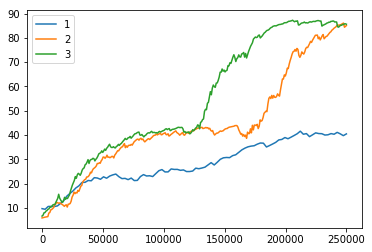
\includegraphics[scale=0.8]{bilder/seaquestprepro}
\caption{Seaquest for default settings \textbf{(1)}, changed hyperparameters \textbf{(2)} and changed hyperparameters with custom preprocessing \textbf{(3)}. A replay ratio of 2 was used for all 3 runs.}
\end{figure}

By applying a minimal individual preprocessing to the Seaquest environment, and slightly adjusted hyperparameters, we managed to both accelerate the learning process and break through the local maximum the learning agents got stuck on in the previous tests.

Even though the results indicate an improved performance for the individually preprocessed environment, a clear statement cannot be made, because the change in hyperparameters managed to outperform the default settings and break through the local optimum as well.

\section{Adversial Attacks}

\section{Conclusion}